\documentclass[11pt]{report}
\title{HW1}

%-----------Packeges---------------%
\usepackage{amsmath}
\usepackage{amssymb}
\usepackage{amsfonts}
\usepackage{tocloft}
\usepackage{float}
\usepackage{graphicx}
\usepackage[bookmarks=true]{hyperref}
\usepackage{fancyhdr}


%----------Definition & Theorem----%
\newtheorem{definition}{Definition}[subsection]
\newtheorem{theorem}{Theorem}[subsection]
\newtheorem{proposition}{Proposition}[subsection]
\newtheorem{lemma}{Lemma}[subsection]
\newtheorem{corollary}{Corollary}[subsection]


\pagestyle{fancy}
\fancyhead[L]{Math 417}
\fancyhead[C]{HW1}
\fancyhead[R]{Lanxiao Bai(lbai5)}
\begin{document}
\paragraph{1.3.1}
List the symmetries of an equilateral triangular plate (there are six) and work out the multiplication table for the symmetries.\\

\textbf{Solution:} There're 6 symmetries in total for an equilalateral triangular plate as listed following:
    \begin{enumerate}
        \item 3 Rotational symmetries: $e, r, r^2$;
        \item 3 Reflectional symmetries: $a, b=ra, c=r^2a$.
    \end{enumerate}
And the multiplication table is as following:
\begin{table}[!hbp]
    \centering
    \begin{tabular}{c || c | c | c || c | c | c ||}
        
        & $e$ & $r$ & $r^2$ & $a$ & $b$ & $c$\\
        \hline
        \hline
           
           $e$ & $e$ & $r$ & $r^2$ & $a$ & $b$ & $c$\\
        \hline
           $r$ & $r$ & $r^2$ & $e$ & $b$ & $c$ & $a$\\
        \hline
           $r^2$ & $r^2$ & $e$ & $r$ & $c$ & $a$ & $b$\\
        \hline
        \hline
            $a$ & $a$ & $b$ & $c$ & $e$ & $r$ & $r^2$\\
        \hline
            $b$ & $b$ & $c$ & $a$ & $r^2$ & $e$ & $r$\\
        \hline
            $c$ & $c$ & $a$ & $b$ & $r$ & $r^2$ & $e$\\        
        \hline\hline
    \end{tabular}
    \caption{Table of Multiplication for Equilateral Triangle}
\end{table}


\paragraph{1.3.3}
    \subparagraph{(a)}
        \textbf{Solution:} 
        \begin{figure}[H]
        \begin{center}
        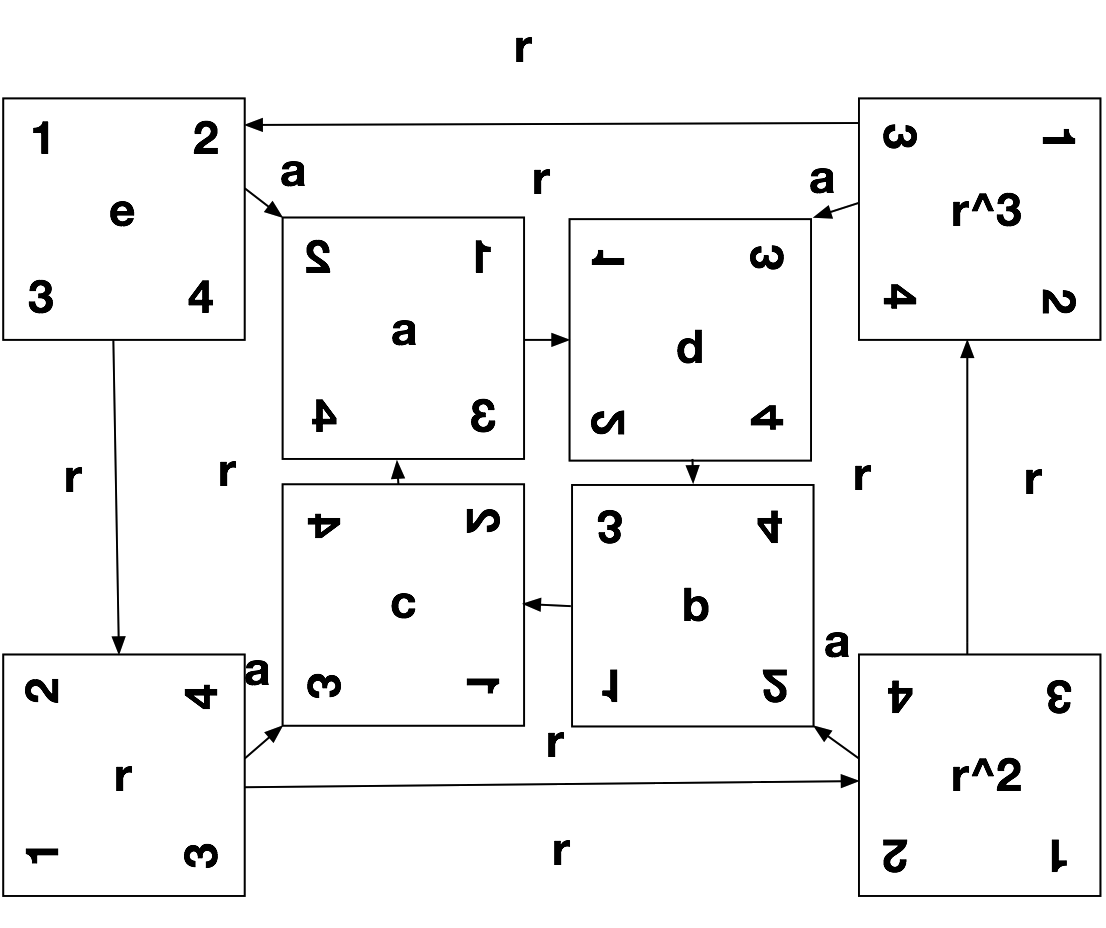
\includegraphics[width=7cm]{./imgs/square_symmetry.png}
        \caption{$D_4$ Symmetry}
        \end{center}
    \end{figure}
    As the graph above has shown, it's clear that,
        \begin{equation} a = a \end{equation}
        \begin{equation} b = ar^2
\end{equation}
        \begin{equation} c = ar^3
\end{equation}
        \begin{equation} d = ar
\end{equation}

    \subparagraph{(b)}
    \textbf{Solution:} According to equation (3), $ar = d$. And as the graph has shown, that $r^{-1}a = d = r^3a$. 
    
    As a result, $ar = r^{-1}a = r^3a$ is verified.
    \subparagraph{(c)} \textbf{Claim:} $\forall k \in \mathbb{Z}$, $ar^k = r^{-k}a$.\\
    
    \textbf{Proof:} Since $ar^k = r^{-k}a \Leftrightarrow r^kar^kr^{-k} = r^kr^{-k}ar^{-k} \Leftrightarrow r^ka = ar^{-k} \Leftrightarrow ar^{-k} = r^ka$, we have $\forall k \in \mathbb{Z}$, $ar^k = r^{-k}a \Leftrightarrow \forall k \in \mathbb{Z}^*$, $ar^k = r^{-k}a$.
    
    When $k = 0$, $ar^0 = ae = ea = r^0a$ is obvious by the definition of e. 
    
    Suppose when $ k = m \in \mathbb{Z}^*$, $ar^m = r^{-m}a$.
    
    Then when $k = m + 1 \in \mathbb{Z}^*$, $ar^k = ar^{m+1} = ar^mr = (r^{-m}a)r = r^{-1}(r^{-m}a) = (r^{-1}r^{-m})a = r^{-(m+1)}a = r^{-k}a$.
    
    According to the Principle of Mathematical Induction, the claim is proved.
    
    \subparagraph{(d)} \textbf{Solution:} In the group of $G = {e, r, r^2, r^3, a, b, c, d}$, any element can be expressed in the form of $r^ma^n$, $0 \leq m \leq 3$ and $n = 0$ or $1$. For arbitary elements $e_1, e_2, ..., e_k \in G$, product \[P = \prod_{i = 0}^k e_i = \prod_{i = 0}^k r^{m_i}a^{n_i}=r^{\sum_{i=1}^k m_i}a^{\sum_{i=1}^k n_i}\]
    And with the rules we verified in question (b) and (c), $r^k = r^{k\mod 4}$ and $a^k = a$(if k is odd) or $e$(if k is even), so $r^{\sum_{i=1}^k m_i}a^{\sum_{i=1}^k n_i}$ can be reduced to the form of $r^ma^n$, $0 \leq m \leq 3$ and $n = 0$ or $1$.
    
    As a result, these relations suffice to compute any product.
\paragraph{1.4.2}
\textbf{Solution:} In this problem, we need to figure out the coefficiencies in the following function:
    \[\left\{\begin{array}{l} x_2 = w_{11} \cdot x_1 + w_{12} \cdot y_1 \\ y_2 = w_{21} \cdot x_1 + w_{22} \cdot y_1 \end{array} \right.\]
    which can be rewrite with matrix:
    \[\left(\begin{array}{l} x_2 \\ y_2 \end{array} \right) = \left(\begin{array}{ll} w_{11} & w_{12} \\ w_{21} & w_{22} \end{array} \right) \cdot \left(\begin{array}{l} x_1 \\ y_1 \end{array} \right)\]
    So we can start with those 3 rotational symmetries: as it was demostrated in linear algebra, the matrix that rotate a vector $\theta$ radian is \[\left(\begin{array}{rrr} \cos\theta &  -\sin\theta & 0\\ \sin\theta & \cos\theta & 0 \\ 0 & 0 & 1 \end{array} \right)\]. As a result, 
    \begin{itemize}
        \item \[e = \left(\begin{array}{rrr} 1 & 0 & 0\\ 0 & 1 & 0 \\ 0 & 0 & 1\end{array} \right)\]
        \item \[r = \left(\begin{array}{rrr} -\frac{1}{2} & -\frac{\sqrt{3}}{2} & 0 \\  \frac{\sqrt{3}}{2} & -\frac{1}{2} & 0 \\ 0 & 0 & 1 \end{array} \right)\]
        \item \[r^2 = \left(\begin{array}{rrr} -\frac{1}{2} &\frac{\sqrt{3}}{2} & 0 \\  -\frac{\sqrt{3}}{2} & -\frac{1}{2} & 0 \\ 0 & 0 & 1\end{array} \right)\]
    \end{itemize}
    And since the question gives the 3 vertices as $(1, 0, 0), (-1/2, \sqrt{3}/2, 0), (-1/2, -\sqrt{3}/2, 0)$, we can give the matrices of the 3 reflectional are:
    \begin{itemize}
        \item \[a = \left(\begin{array}{rrr} -1 & 0 & 0 \\ 0 & 1 & 0\\ 0 & 0 & 0 \end{array} \right)\]
        \item \[b = ar = \left(\begin{array}{rrr} \frac{1}{2} & -\frac{\sqrt{3}}{2} & 0 \\  -\frac{\sqrt{3}}{2} & -\frac{1}{2} & 0 \\ 0 & 0 & 1\end{array} \right)\]
        \item \[c = br = \left(\begin{array}{rrr} -\frac{1}{2} & \frac{\sqrt{3}}{2} & 0 \\  \frac{\sqrt{3}}{2} & -\frac{1}{2} & 0 \\ 0 & 0 & 1\end{array} \right)\]
    \end{itemize}

\paragraph{B.4} \textbf{Solution:} Let $C = A \cap B$, then $(A \cup B) \setminus (A \cap B) = (A \cup B) \setminus C = (A \setminus C) \cap (B \setminus C) = (A \setminus B) \cup (B \setminus A)$
\paragraph{E.1} \textbf{Claim:}  $\forall S, T \in Hom_K(K^n, K^m), \alpha \in K, [S + T] = [S] + [T]$ and $[\alpha T] = \alpha [T]$.\\

\textbf{Proof:} Since $S, T \in Hom_K(K^n, K^m)$, $S, T$ are $m \times n$ matrices. So they are able to be added. $[S + T]\textbf{x} = (S + T)(\textbf{x}) = S(\textbf{x}) + T(\textbf{x}) = [S]\textbf{x} + [T]{\textbf{x}} = ([S] + [T])\textbf{x}$, so we can multiply $x^{-1}$ on both sides of the equation and get \[[S + T] = [S] + [T]\]

And similarly, $[\alpha T]\textbf{x} = (\alpha T)(\textbf{x}) = \alpha T(\textbf{x}) = \alpha [T]\textbf{x}$. As a result,
    \[[\alpha T] = \alpha [T]\] 
is proved to be true.

\end{document}
